\section{Reference aircraft}
\paragraph{} The new airport will have two runway with different Airfield reference keys. The International flights thought one, with 4E reference key and the domestic dedicated runway with 4C reference key.

New airport, will absorb around de 40\% of Soekarno-Hatta International Airport air traffic. As it can be seen, the most common code letter is C, but some big planes with code E can also appear. That is why, the new aircraft, despite it will be dedicated domestic flights, will be able to handle big international flights also, Fig. \ref{aircraftDist}.
\begin{figure}[H]
	\centering
	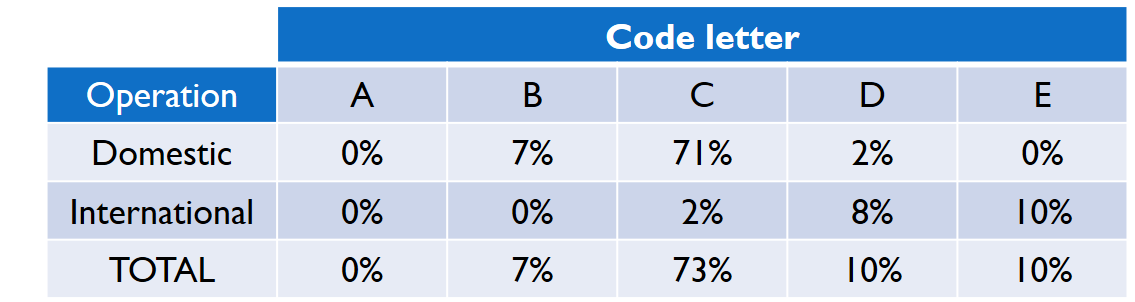
\includegraphics[clip, trim=0.1cm 0.1cm 0.1cm 0.1cm, width=0.8\textwidth]{./images/PROGNOSIS/aircraft/aircraftDist}
	\caption{Soekarno-Hatta International Airport aircraft class distribution.}
	\label{aircraftDist}
\end{figure}

	\subsection{Aircraft type for 4E reference key airfield}
	\paragraph{} A380 is discarded, because the new airport aims to absorb domestic flights mainly but also some international traffic (close range). B777-300 and A330-300, are found to be the bigger planes with higher requirements to operate on the new airport. 
	\begin{figure}[H]
		\centering
		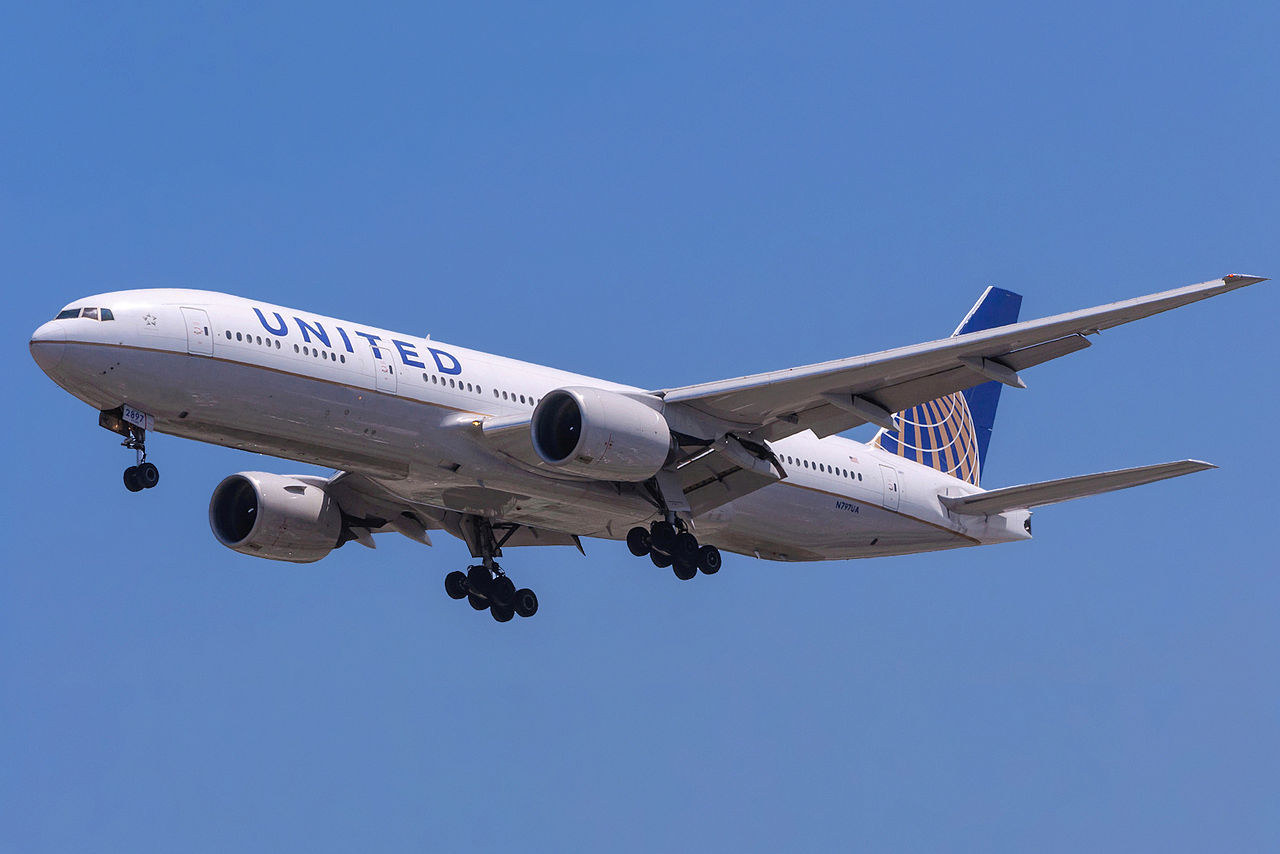
\includegraphics[clip, trim=0cm 0cm 0cm 0cm, width=0.8\textwidth]{./images/PROGNOSIS/aircraft/b777}
		\caption{Boeing 777-300}
		\label{b777}
	\end{figure}
	\begin{figure}[H]
		\centering
		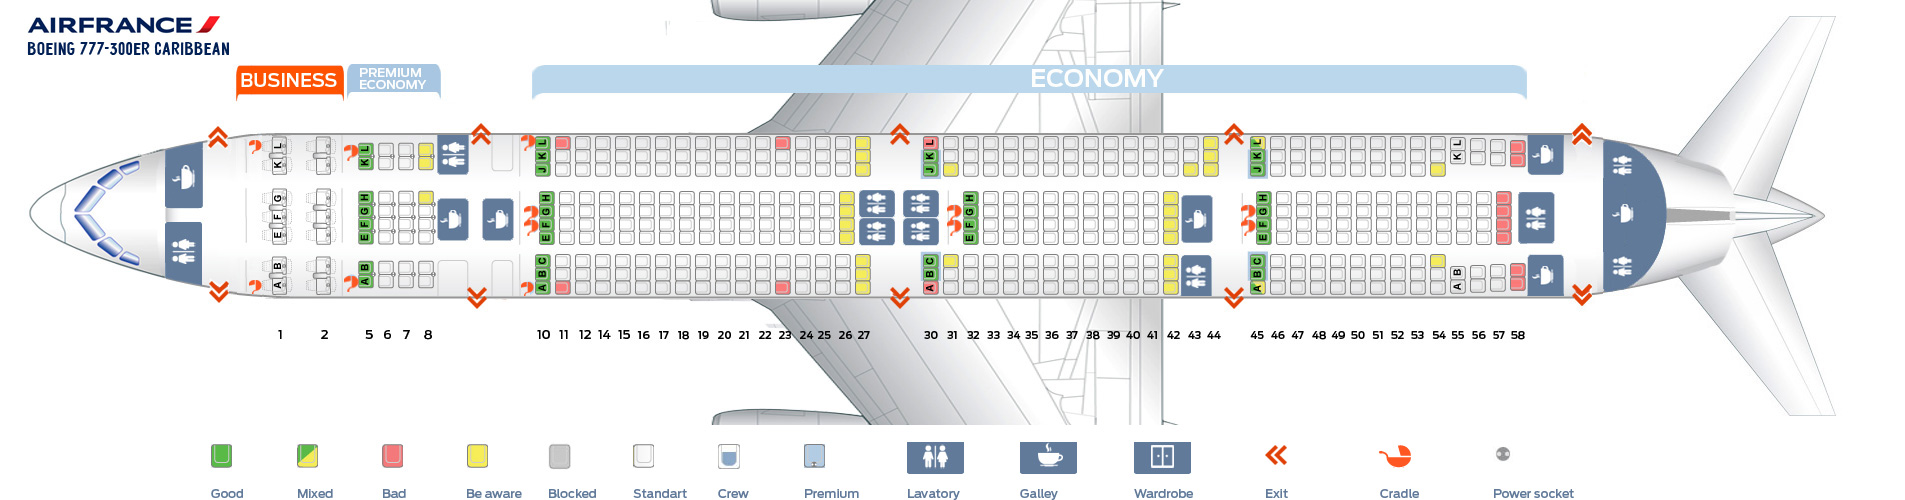
\includegraphics[clip, trim=0cm 0cm 0cm 0cm, width=0.8\textwidth]{./images/PROGNOSIS/aircraft/b777seats}
		\caption{Boeing 777-300, seats distribution.}
		\label{b777seats}
	\end{figure}

	On the one hand, B777-300, on standard configuration carries 350 passengers and have a range of 5,240 nautical miles (9,700 km).

	\begin{figure}[H]
		\centering
		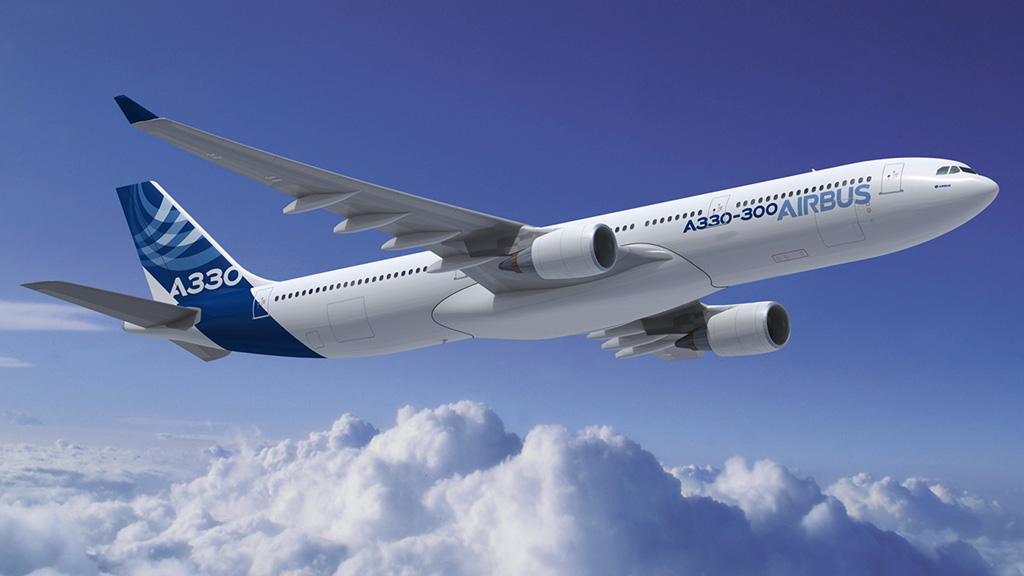
\includegraphics[clip, trim=0cm 0cm 0cm 0cm, width=0.8\textwidth]{./images/PROGNOSIS/aircraft/a330}
		\caption{Airbus 330-300}
		\label{a330}
	\end{figure}
	\begin{figure}[H]
		\centering
		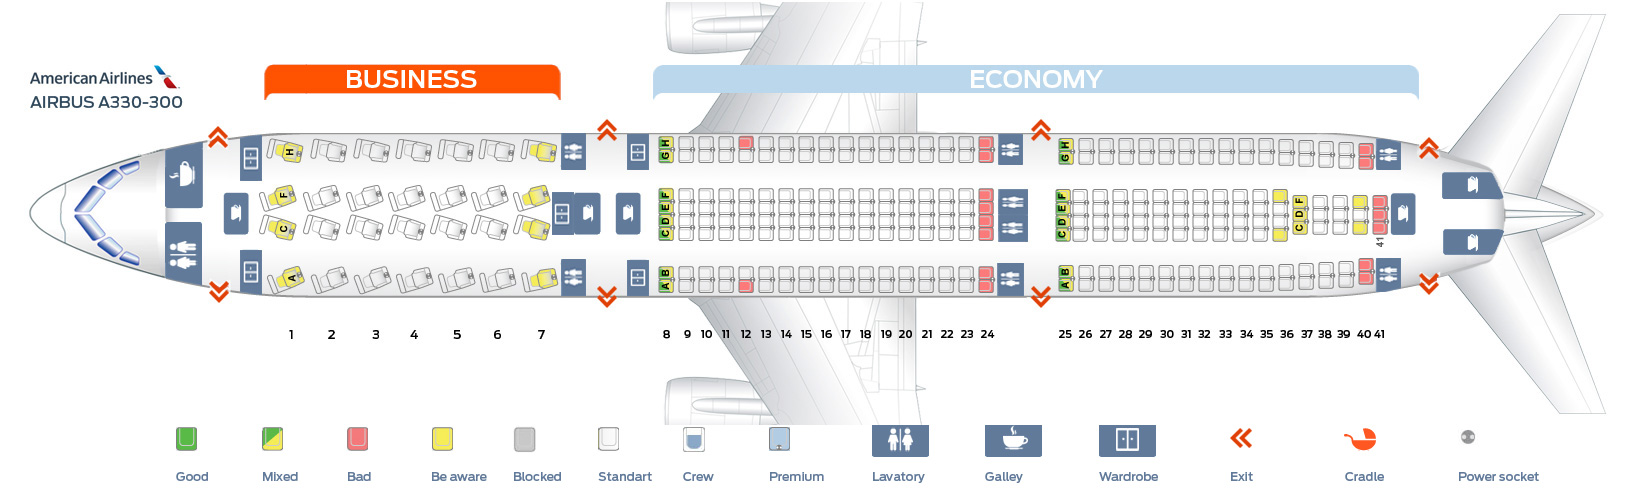
\includegraphics[clip, trim=0cm 0cm 0cm 0cm, width=0.8\textwidth]{./images/PROGNOSIS/aircraft/a330seats}
		\caption{Airbus 330-300, seats distribution.}
		\label{a330seats}
	\end{figure}

	On the other hand, A330-300, on standard configuration carries 270 passengers and have a range of 11750km.
	
	\subsection{Aircraft type for 4C reference key airfield}
	\paragraph{} B737-800, is chosen because have longer take-off requirements compared to A320 and other smalls planes, operating on the Jakarta area.
	\begin{figure}[H]
		\centering
		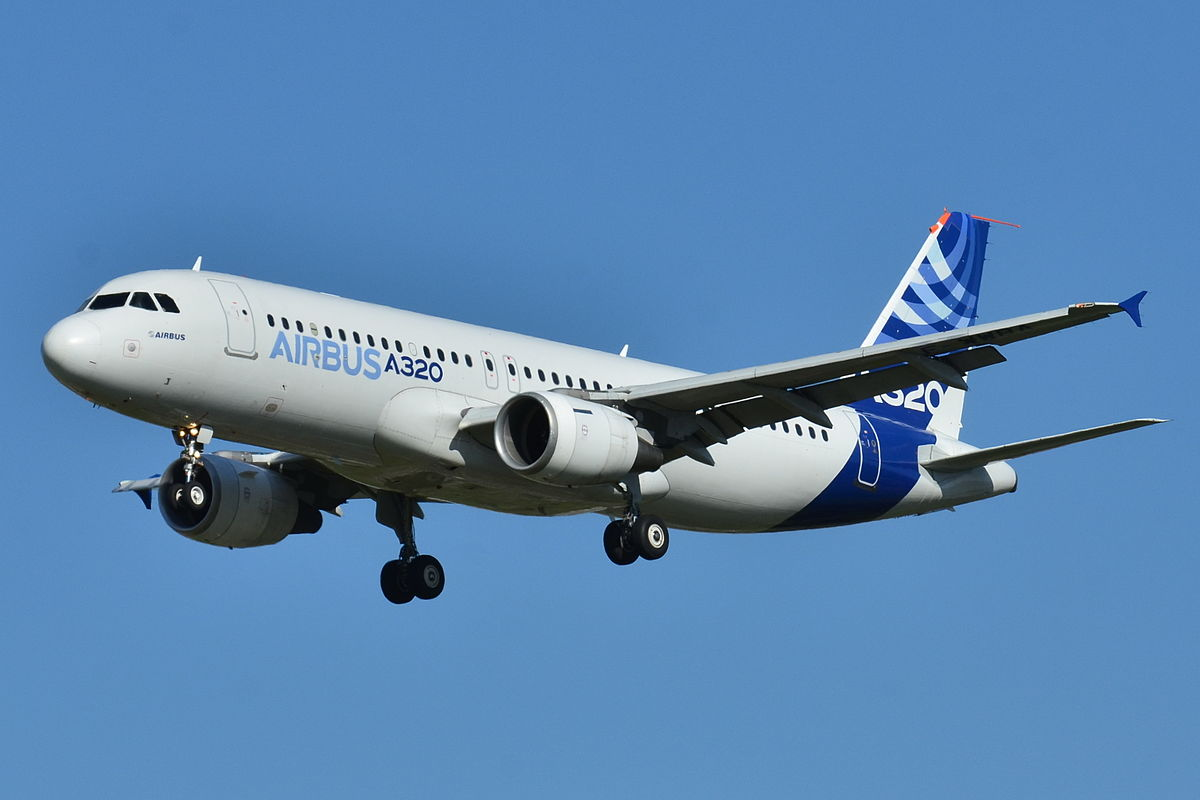
\includegraphics[clip, trim=0cm 0cm 0cm 0cm, width=0.8\textwidth]{./images/PROGNOSIS/aircraft/a320}
		\caption{Airbus 320}
		\label{a320}
	\end{figure}
	\begin{figure}[H]
		\centering
		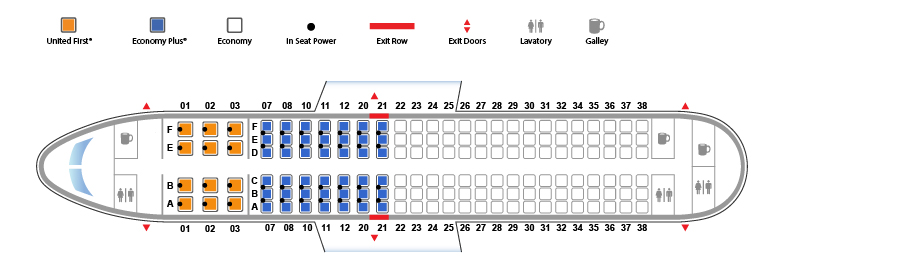
\includegraphics[clip, trim=0cm 0cm 0cm 0cm, width=0.8\textwidth]{./images/PROGNOSIS/aircraft/a320seats}
		\caption{Airbus 320, seats distribution.}
		\label{a320seats}
	\end{figure}

	A330-300, on standard configuration carries 150 passengers and have a range of 6100 km.
	
	\subsection{Conclusions}
	\paragraph{} Comparing the aircraft types for 4E reference key airfield, is possible to state that both two planes have almost identical operating conditions. The interesting facts that will be studied on the report will be: the biggest of the two MTOW for determining the runway length (Air side report) and the passengers seats configurations around Jakarta for determining the average passengers per plane.
	
	This planes will both operate as regional airlines and as short international flights between nearby countries.
	
	\paragraph{} Aircraft type for 4C reference key airfield will operate as regional airliner, with planes that will allocate passengers volums between 150 -200 depending on the configuration. Selected number of passengers will be explained on the following prognosis study.
	